\section{Generation and Management of M3D-C$^{1}$ Meshes}
\subsection{Introduction}

This section describes the methods used to generate M3D-C$^{1}$ meshes for Tokamak geometries. This process involves the use of specific software and interaction with several files that contain the associated geometry and mesh information.

The process of generating M3D-C$^{1}$ meshes involves the use of two software libraries. They are: 
\begin{itemize}
\item m3dc1\_meshgen coordinates the process of generating the an initial M3D-C$^{1}$
\item	Simmetrix provides a set of tools and libraries for engineering simulation including a state-of-art mesh generation. For more information, visit \href{http://simmetrix.com}{http://simmetrix.com}. The Simmetrix library is used to generate the M3D-C$^{1}$ meshes. The Simmetrix meshing library is used by m3dc1\_meshgen for the actual mesh generation. The Simmetrix GUI can be used after the execution of m3dc1\_meshgen to apply additional mesh controls for the generation of meshes with different mesh gradations. 
\item PUMI is a parallel mesh infrastructure toolkit developed at SCOREC, RPI. For more information, visit \href{http://www.scorec.rpi.edu/pumi}{http://www.scorec.rpi.edu/pumi}. The PUMI library is used to manage the mesh information as it is processed and within the M3D-C$^{1}$ code.
\end{itemize}

There are a number of files involved with housing the geometry and mesh information. 

The model file extensions referred in this document is the following
\begin{itemize}
\item \texttt{.smd}: Simmetrix-readable binary format model file  
\newline  The model generated with Simmetrix is saved in this format.
\item \texttt{.dmg}: PUMI-readable binary format model file
\newline	The model generated from PUMI mesh
\item	\texttt{.txt}: M3D-C$^{1}$-readable ascii format model file 
\newline	The model is generated from mesh generation tool (See Section~\ref{ch:mesh-gen})
\end{itemize}

The mesh file extensions referred in this document is the following.
\begin{itemize}
\item	\texttt{.sms}: Simmetrix-readable binary format mesh file
\begin{itemize}
\item	The mesh generated with Simmetrix is saved in this format.
\item	If a mesh is serial (1-part), the mesh file doesn't have a number before the extension
\item	If a mesh is distributed (\texttt{P}-part, P$>$1), the mesh file has a number before the extension to represent the global part ID.
\end{itemize}
\item	\texttt{.smb}: PUMI-readable binary format mesh file
\begin{itemize}
\item	This format is used in M3D-C$^{1}$ to import/export a mesh
\item	No matter if a mesh is serial (1-part) or distributed (\texttt{P}-part, P$>$1), the mesh file has a number before the extension to represent the global part ID.
\end{itemize}
\item \texttt{.vtu/pvtu}: binary format mesh file for visualization with Paraview. For more information, visit \href{http://paraview.org}{http://paraview.org}.
\end{itemize}

An overview of the Model/Mesh requirements for the M3D-C$^{1}$ mesh generation process are as follows:
\begin{itemize}
\item	The model and mesh shall be generated as described in Section~\ref{ch:mesh-gen}.
\item	The mesh file must be PUMI-readable \texttt{.smb} file. Note that a mesh file name contains a number before the extension (.smb) to denote a global part ID.
\item	The model and mesh file must be present in the work directory
\item	The name of model and mesh file must be specified in \texttt{C1input} file in the work directory
\begin{itemize}
\item	mesh\_model = model\_file
\item	mesh\_filename = mesh\_file.smb (NOTE: do not specify a number before the file extension)
\end{itemize}
\item In a 2D run with \texttt{P} processes, there should be \texttt{P} mesh files with part ID from \texttt{0} to \texttt{P-1}
\item	In a 3D run with \texttt{P$\times$N} processes where 2D mesh is distributed to \texttt{P} parts, 
\begin{itemize}
\item	there should be \texttt{P} mesh files with part ID from \texttt{0} to \texttt{P-1}
\item	in \texttt{C1input} file, specify \texttt{nplanes} to \texttt{N} (e.g. nplanes=8), where \texttt{nplanes} describes how many 2D mesh copies to be loaded
\item	the M3D-C$^{1}$ code should be compiled with options \texttt{"3D=1, MAX\_PTS=60"}.
\end{itemize}
\end{itemize}

The rest of this section is organized as follows: Section \ref{ch:mesh-gen} describes a mesh generation program \texttt{m3dc1\_meshgen}. Section \ref{ch:mesh-ptn} presents a mesh partitioning program \texttt{"split\_smb"} and \texttt{"collapse"} which changes the number of parts of the mesh. For how to visualize a mesh with \texttt{Paraview}, see Appendix~\ref{ch:app-paraview}.

%%%%%%%%%%%%%%%%%%%%%%%%%%%%%%%%%%%%%%%%%
\subsection{Mesh Generation}
\label{ch:mesh-gen}
%%%%%%%%%%%%%%%%%%%%%%%%%%%%%%%%%%%%%%%%%

Two programs \texttt{m3dc1\_meshgen} and \texttt{polar\_meshgen} are provided for mesh generation. \texttt{m3dc1\_meshgen} is used to define the tokamak cross section geometry and an initial mesh.  \texttt{polar\_meshgen} generates a mesh based on equilibria transfered from the PPPL JSOLVER code. As the mesh generation programs require Simmetrix licence and proper enviroment settings, the user should load Simmetrix modules as the following:
\newline\newline
\texttt{
module load simmodsuite/version simmodeler/version
}
\newline\newline
As of today (July 11, 2022), the latest Simmetrix modules are \texttt{simmodsuite/16.0-220226} and \texttt{simmodeler/10.0-220226}.
\newline\newline
Two mesh generation programs are available only on PPPL Portal in the following location:
\newline\newline
\texttt{/p/tsc/m3dc1/lib/SCORECLib/rhel\_ver/intel\_ver-openmp\_ver/simmodsuite\_ver/bin}
\newline\newline
For instance, for Centos7, intel/2019.u3 openmpi/4.0.3, and simmodsuite/16.0-210626, the mesh generation programs are available in 
\newline\newline
\texttt{/p/tsc/m3dc1/lib/SCORECLib/rhel7/intel2019u3-openmpi4.0.3/16.0-220226/bin}


%%%%%%%%%%%%%%%%%%%%%%%%%%%%%%%%%%%%%%%%%
\subsubsection{m3dc1\_meshgen}
%%%%%%%%%%%%%%%%%%%%%%%%%%%%%%%%%%%%%%%%%
\texttt{m3dc1\_meshgen} requires an ascii input file of arbitrary name that contains the following parameters.

\begin{itemize}
\item numBdry: number of boundary file defined by peice-wise linear points (default: 0)
\item bdryFile: boundary file name. Each boundary file corresponds to a loop in PUMI. Each loop has a unique ID starting from 1.
\item numRgn: number of region (geometric face)
\item rgnBdry: information to define each region. This requires the number of loops and loop id(s).
\item outFile: output file name to save model and mesh
\item meshSize: relative mesh size for each region (default 0.05)
\item useVacuum: if 1, create a vacuum wall (default 0)
\item useVacuumParams: if 1, create a parameterized vacuum wall (default 0)
If useVacuum=0, this parameter is ignored.
\item vacuumParams: five doubles to describe parameterized vacuum wall. Required if useVacuumParams=1.
If useVacuum=0 or useVacuumParams=0, this parameter is ignored. 
\item adjustVacuumParams: if 1, multiply coordinates and parametric values of nodes on vacuum wall by vacuumFactor (default 0). If useVacuum=0 or useVacuumParams=0, this parameter is ignored.
\item vacuumFactor: an optional double value used to multiply coordinates and parametric values of nodes on vacuum wall when adjustVacuumParams=1 (default 2$\times$PI). Valid only if adjustVacuumParams=1.
\item numVacuumPts: optional \# interpolation points on parameterized vacuum wall. Valid only if useVacuumParams=1 (default 20)
\item meshGradationRate: for multiple region model, optional mesh gradation rate (default: 0.3). This value should be greater than or equal to 0.3. Otherwise the mesh will be fine everywhere.
\item resistive-width: for multiple region model without peice-wise boundary points, set the width of resistive wall. If resistive-width=0, only plasma region is created (default 0.02)
\item plasma-offsetX: for multiple region model without peice-wise boundary points, the offset in x direction to the left (default 0.0)
\item plasma-offsetY: for multiple region model without peice-wise boundary points, the offset in y direction to the bottom (default 0.0)
\item vacuum-width: for multiple region model, the width of vacuum region (default 2.5)
\item vacuum-height: for multiple region model, the height of vacuum region (default 4.0) 
\end{itemize}

Locate input parameter file and all files listed as bdryFile (if applicable) in the work folder and do \texttt{m3dc1\_meshgen input\_param\_file}, then the following output will be generated.

\begin{itemize}
\item The output model in three formats
  \begin{itemize}
  \item	$M3D-C^1$-readable \texttt{.txt}
  \item	Simmetrix-readable file \texttt{.smd} and 
  \item	PUMI-readable \texttt{.dmg}
    \begin{itemize}
    \item[$\triangleright$] For modelType 0-2, the model is saved in \texttt{outFile.*}
    \item[$\triangleright$] For modelType 3 with resistive width \texttt{R}, vacuum-width \texttt{W} and vacuum-height \texttt{H}, the model is saved in \texttt{outFile-R-W-H.*}.
    \item[$\triangleright$] For modelType 4 with vacuum-width \texttt{W} and vacuum-height \texttt{H}, the model is saved in \texttt{outFile-W-H.*}.
    \end{itemize}
  \end{itemize}
\item The output mesh in three formats
  \begin{itemize}
  \item Simmetrix-readable\texttt{.sms}
  \item $M3D-C^1$/PUMI readable \texttt{.smb}
  \item Paraview 
    \begin{itemize}
    \item[$\triangleright$] For modelType 0-2 with \# mesh faces \texttt{F}, 
      \begin{itemize}
      \item[-] if \texttt{F} $>$ 1000, the mesh is saved in \texttt{outFile-(F/1000).*}
      \item[-] if \texttt{F} $<$ 1000, the mesh is saved in \texttt{outFile-F.*}
      \end{itemize}
    \item[$\triangleright$] For modelType 3 with \# mesh faces \texttt{F}, resistive width \texttt{R}, vacuum-width \texttt{W}, vacuum-height \texttt{H},
      \begin{itemize}
      \item[-] if \texttt{F} $>$ 1000, the mesh is saved in \texttt{outFile-R-W-H-(F/1000).*}
      \item[-] if \texttt{F} $<$ 1000, the mesh is saved in \texttt{outFile-R-W-H-F.*}
      \end{itemize}
    \item[$\triangleright$] For modelType 4 with \# mesh faces \texttt{F}, vacuum-width \texttt{W} and vacuum-height \texttt{H},
      \begin{itemize}
      \item[-] if \texttt{F} $>$ 1000, the mesh is saved in \texttt{outFile-W-H-(F/1000).*}
      \item[-] if \texttt{F} $<$ 1000, the mesh is saved in \texttt{outFile-W-H-F.*}
      \end{itemize}
    \end{itemize}
  \end{itemize}
\end{itemize}

If the initial mesh is not good enough, run \texttt{simmodeler} to generate a mesh with more meshing controls. See Section~\ref{ch:simmodeler} for detailed instructions.

\begin{verbatim}
numBdry 0
numRgn 1
rgnBdry 1 1
outFile analytic-0.09
meshSize 0.09
useVacuumParams 1
vacuumParams 1.65908 0.46 0.2 -0.02504 0.8
numVacuumPts 20
\end{verbatim}

\begin{figure}
\centering
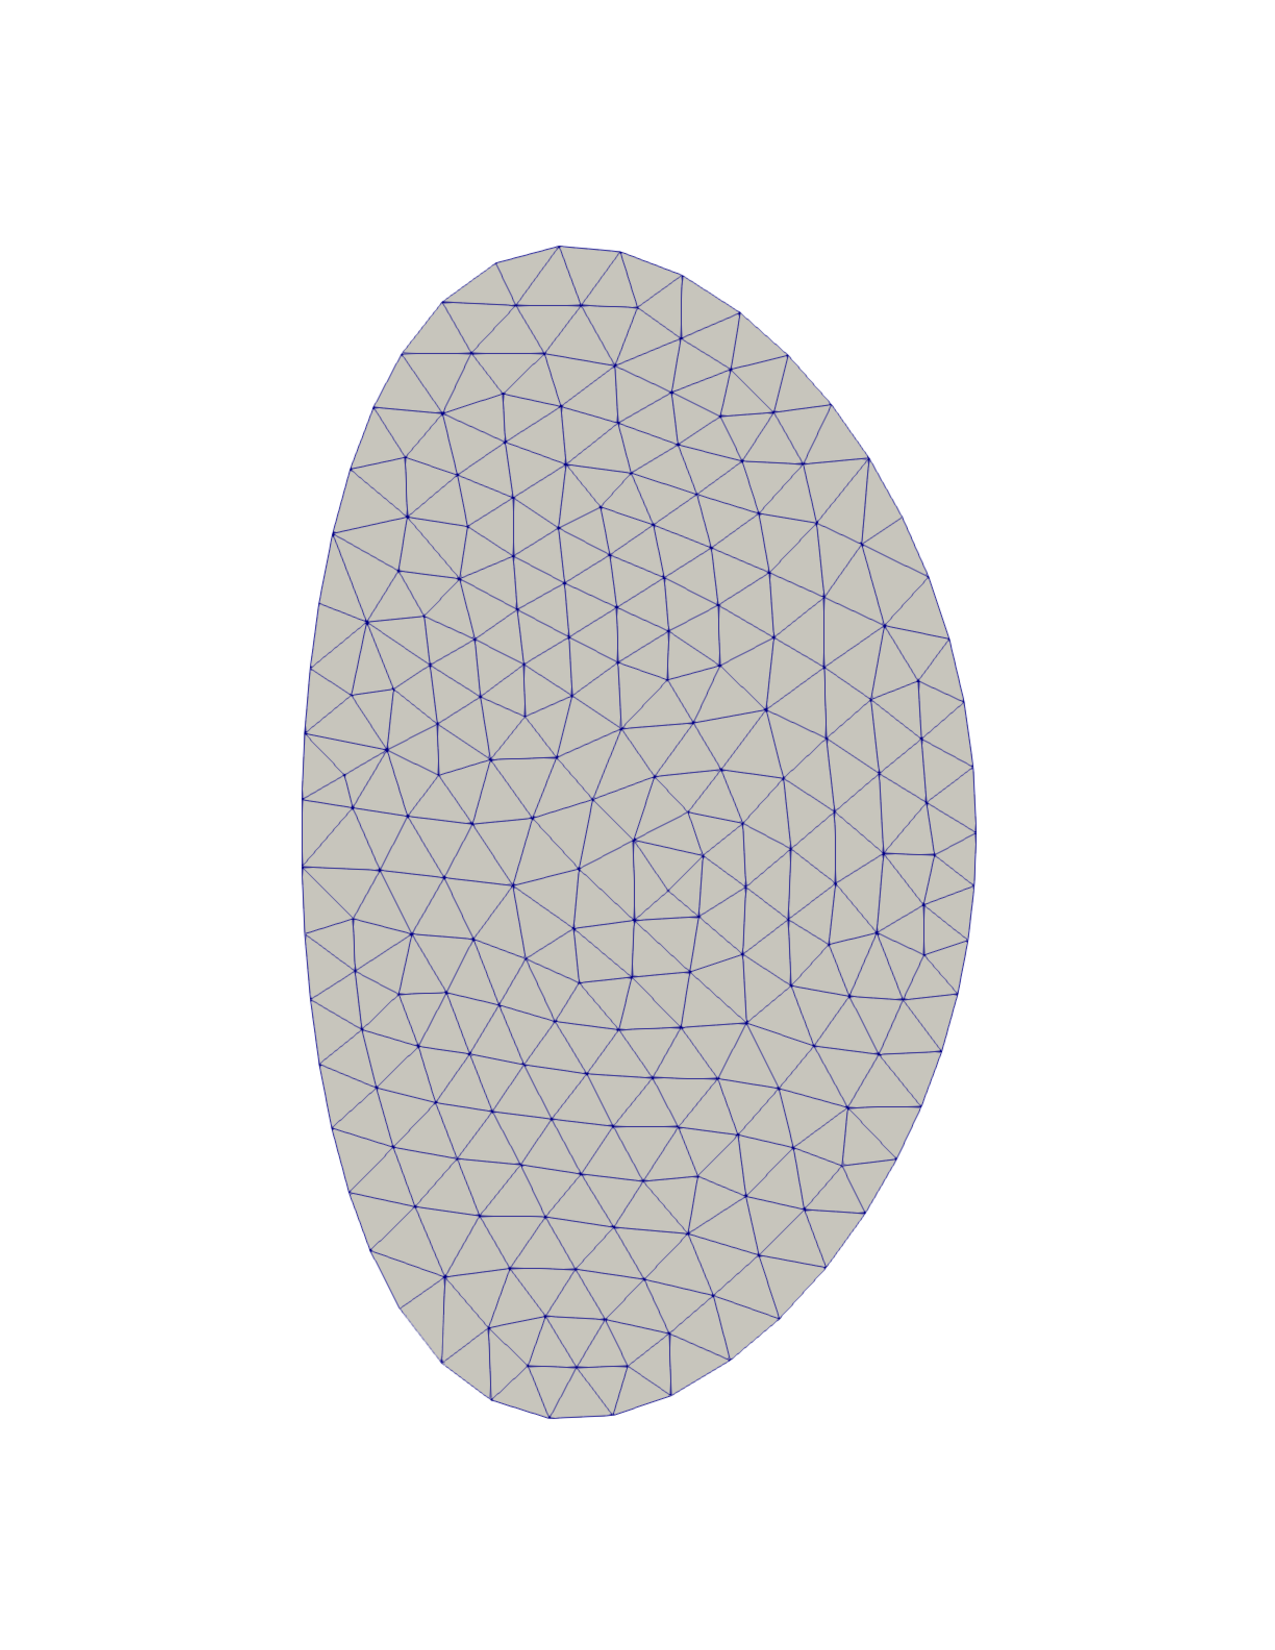
\includegraphics[width=3in]{./figures/meshgen-analytic-20pts-09.pdf}
\caption[Mesh with parameterized vacuum region I]
{A mesh with parameterized vacuum region of 20 interpolation points and mesh size 0.09}
\label{fig:analytic-mesh-1}
\end{figure}

The figure~\ref{fig:analytic-mesh-1} presents the mesh generated by the input file above.

\begin{verbatim}
numBdry 0
numRgn 1
rgnBdry 1 1
outFile analytic-0.05
meshSize 0.05
useVacuumParams 1
vacuumParams 1.65908 0.46 0.2 -0.02504 0.8
numVacuumPts 50
\end{verbatim}

\begin{figure}
\centering
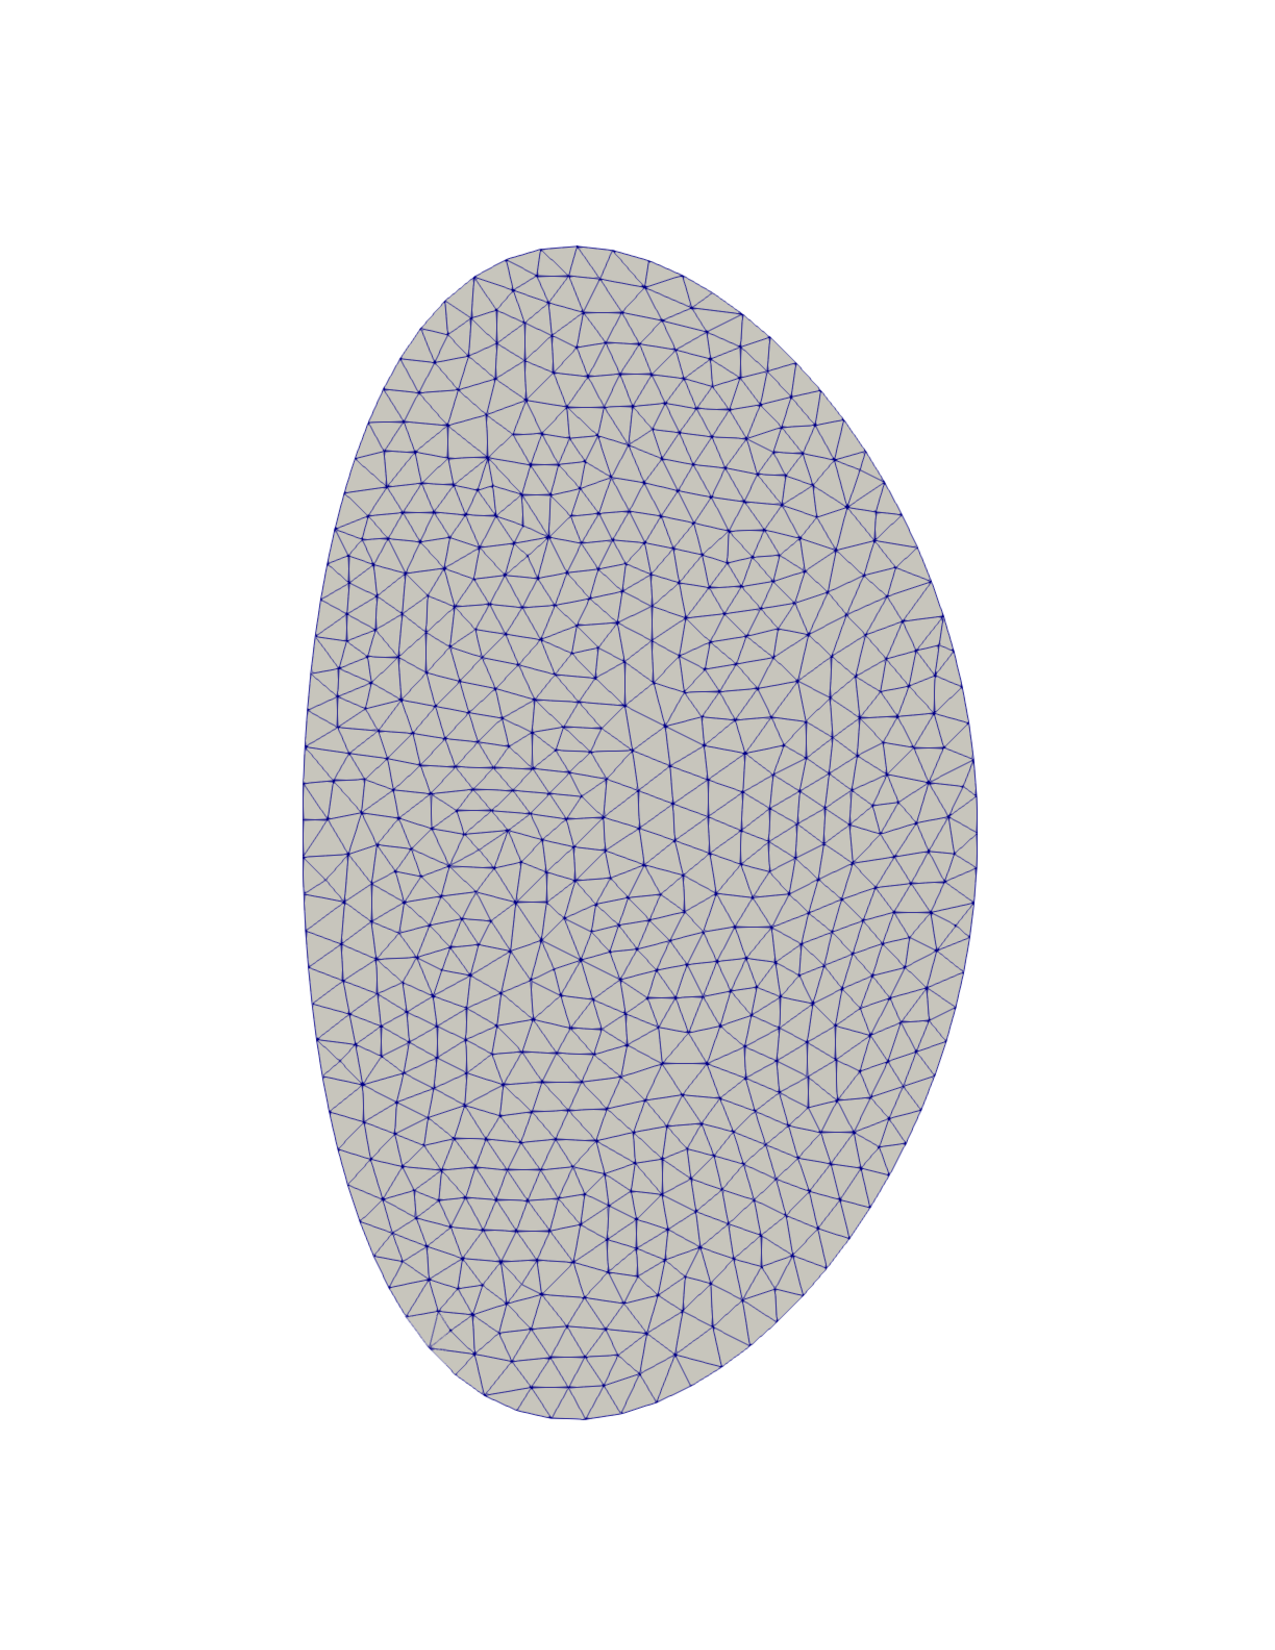
\includegraphics[width=3in]{./figures/meshgen-analytic-50pts-05.pdf}
\caption[Mesh with parameterized vacuum region II]
{A mesh with parameterized vacuum region of 50 interpolation points and mesh size 0.05}
\label{fig:analytic-mesh-2}
\end{figure}

The figure~\ref{fig:analytic-mesh-2} presents the mesh generated by the input file above.

\begin{verbatim}
numBdry 1
bdryFile loop1.dat
numRgn 1
rgnBdry  1 1
outFile input1
useVacuum 0
\end{verbatim}

\begin{figure}
\centering
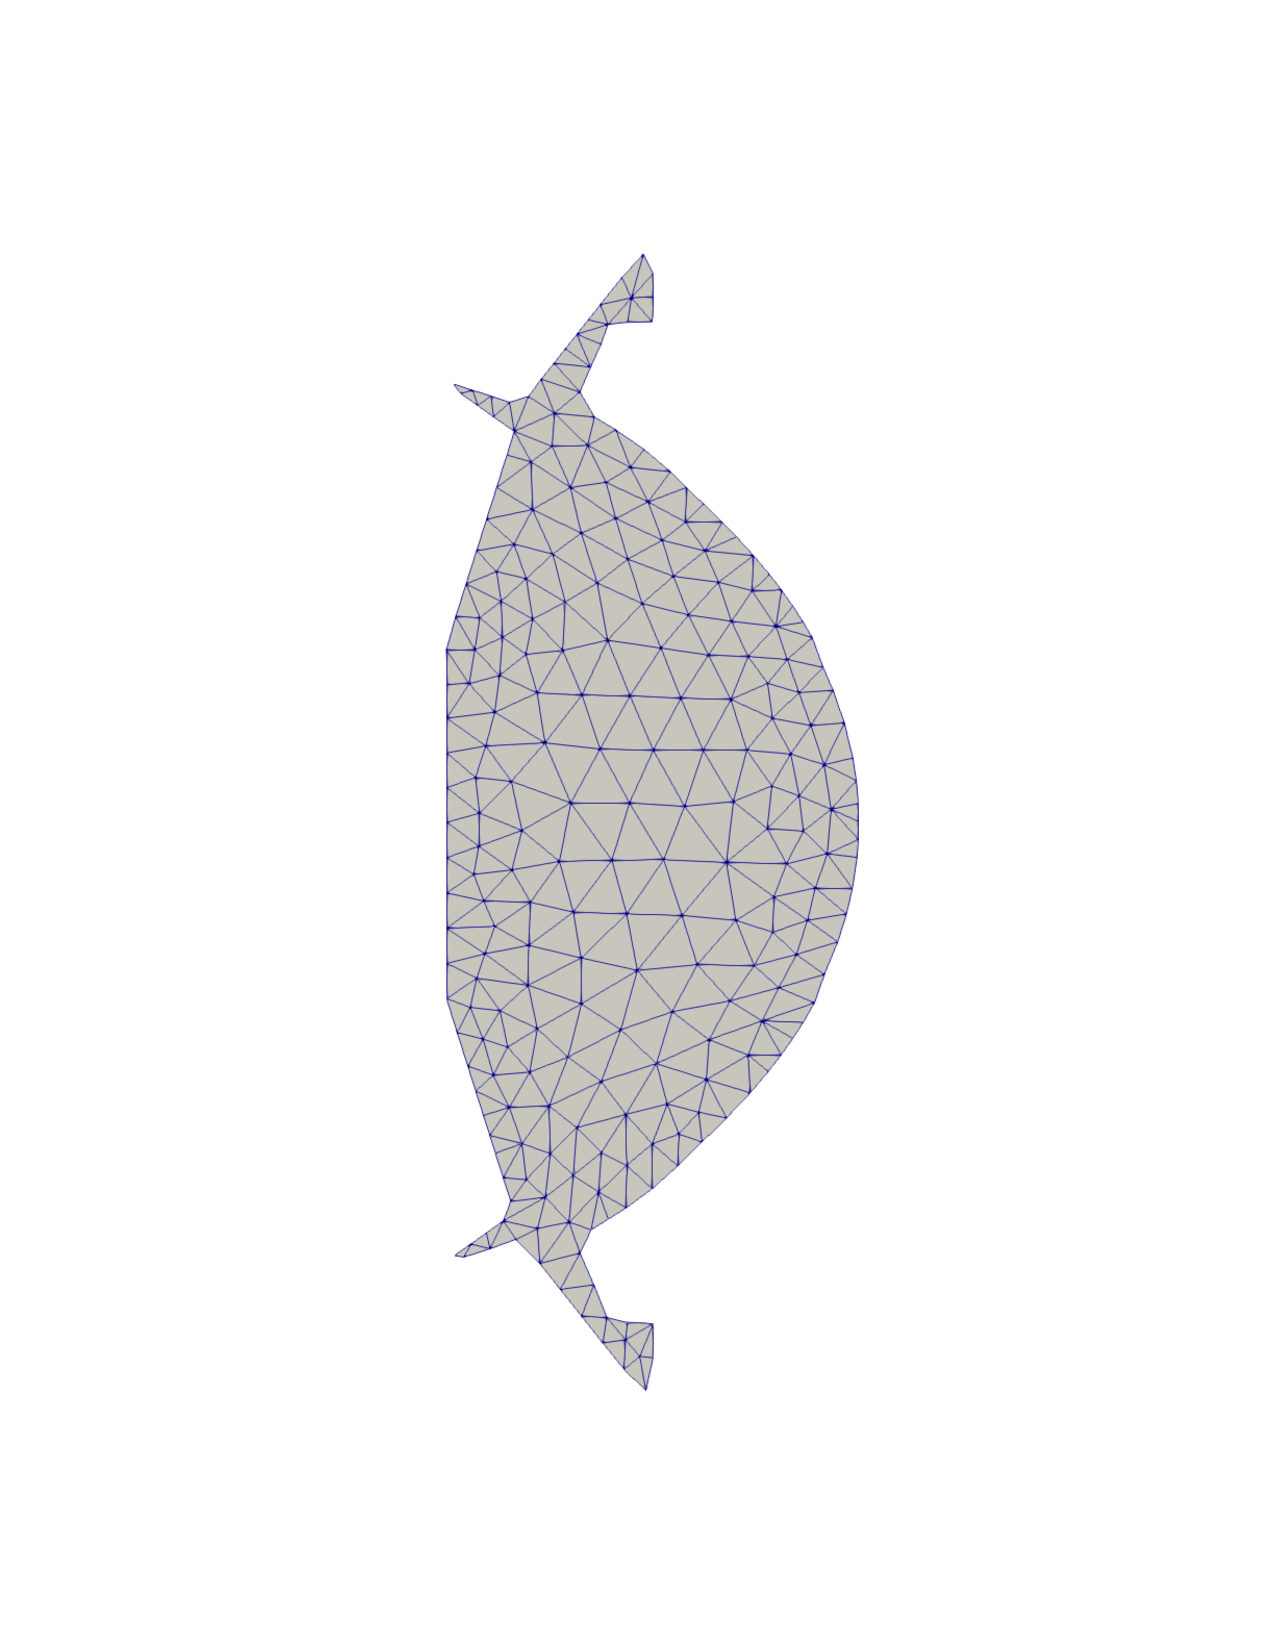
\includegraphics[width=3in]{./figures/meshgen-input1-novacuum.pdf}
\caption[Mesh with one boundary file and no vacuum wall]{Mesh with one boundary file and no vacuum wall}
\label{fig:input1}
\end{figure}

The figure~\ref{fig:input1} presents the mesh generated by the input file above.

\begin{verbatim}
numBdry 1
bdryFile loop1.dat
numRgn 2
rgnBdry  1 1
rgnBdry 2 1 2
outFile input1
meshSize 0.1 0.05 0.5
useVacuum 1
useVacuumParams 1
vacuumParams 1.8 1.5 0.4 0.0 2.5
numVacuumPts 20
\end{verbatim}

\begin{figure}
\centering
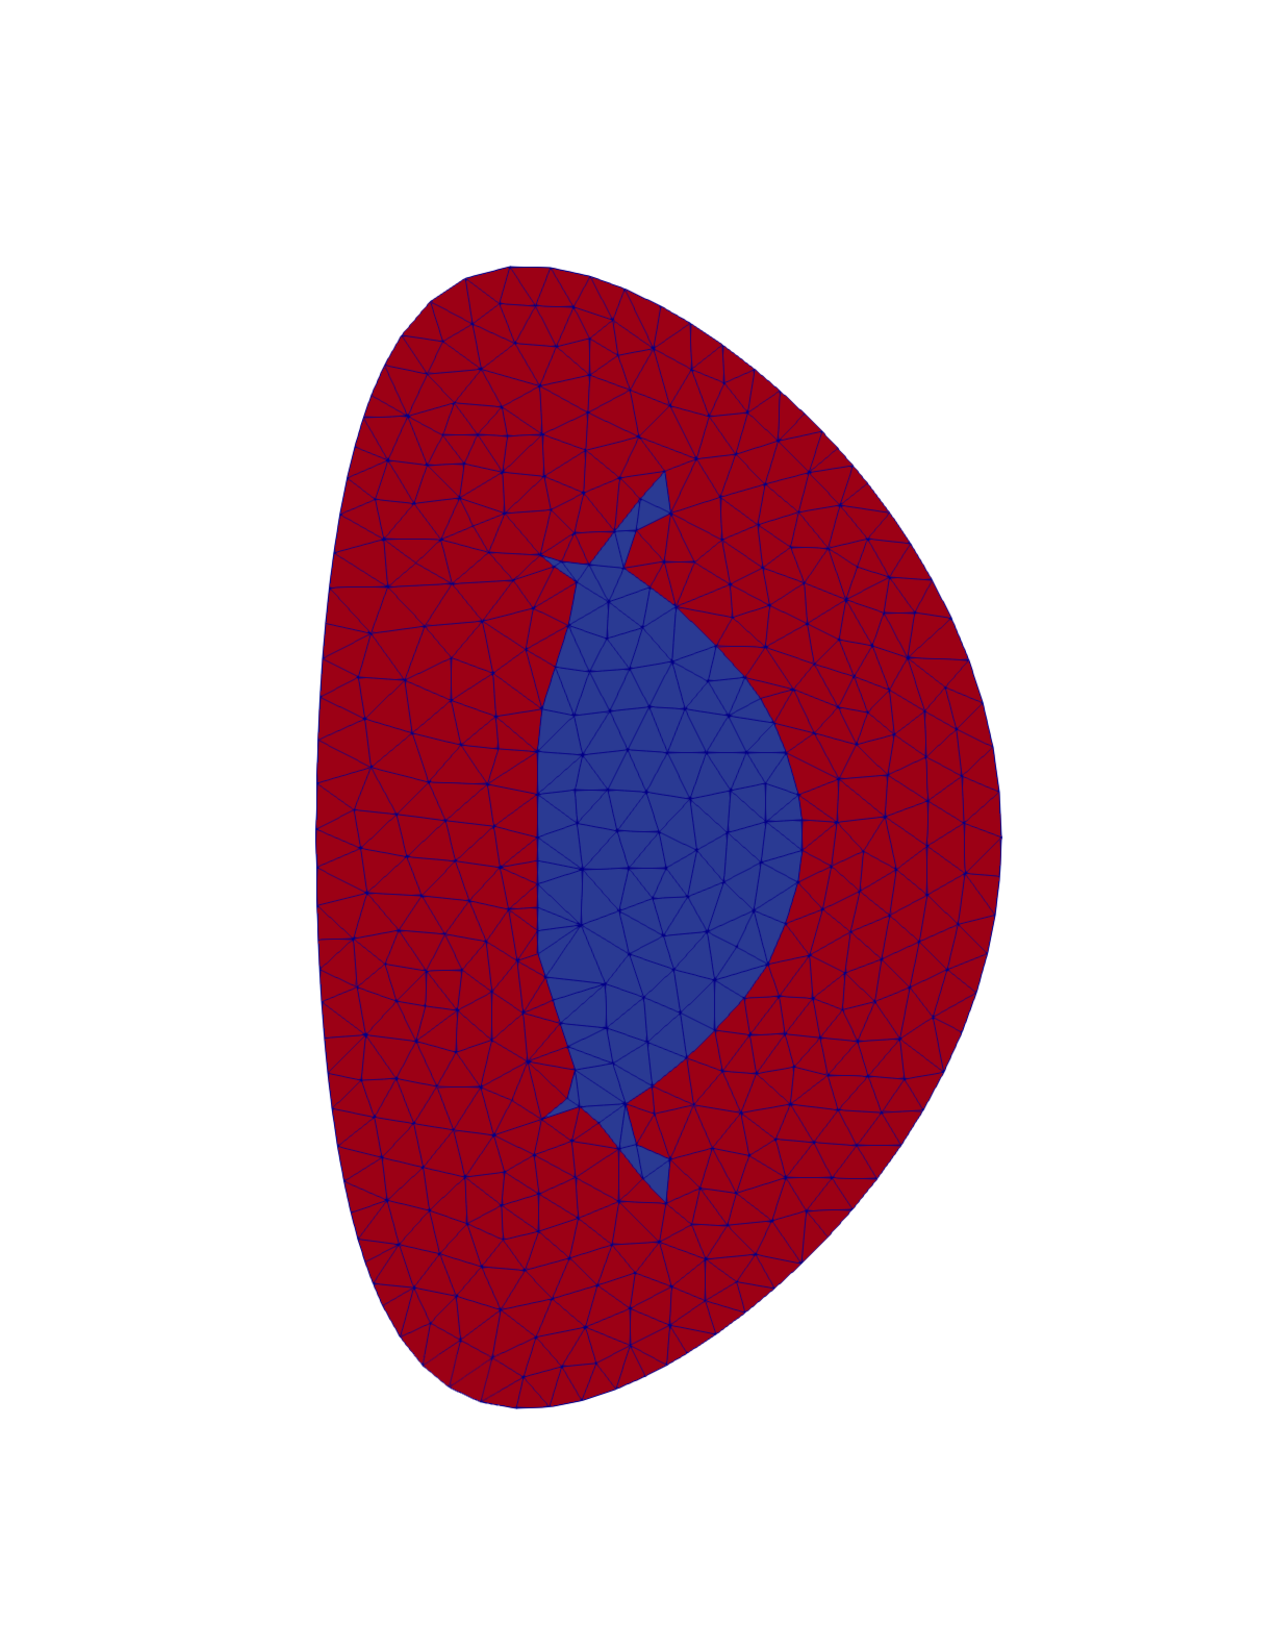
\includegraphics[width=3in]{./figures/meshgen-input1.pdf}
\caption[Mesh with one boundary file and vacuum wall]
{Mesh with one boundary file and vacuum wall}
\label{fig:input1-vacuum}
\end{figure}

The figure~\ref{fig:input1-vacuum} presents the mesh generated by the input file above.

\begin{figure}
\centering
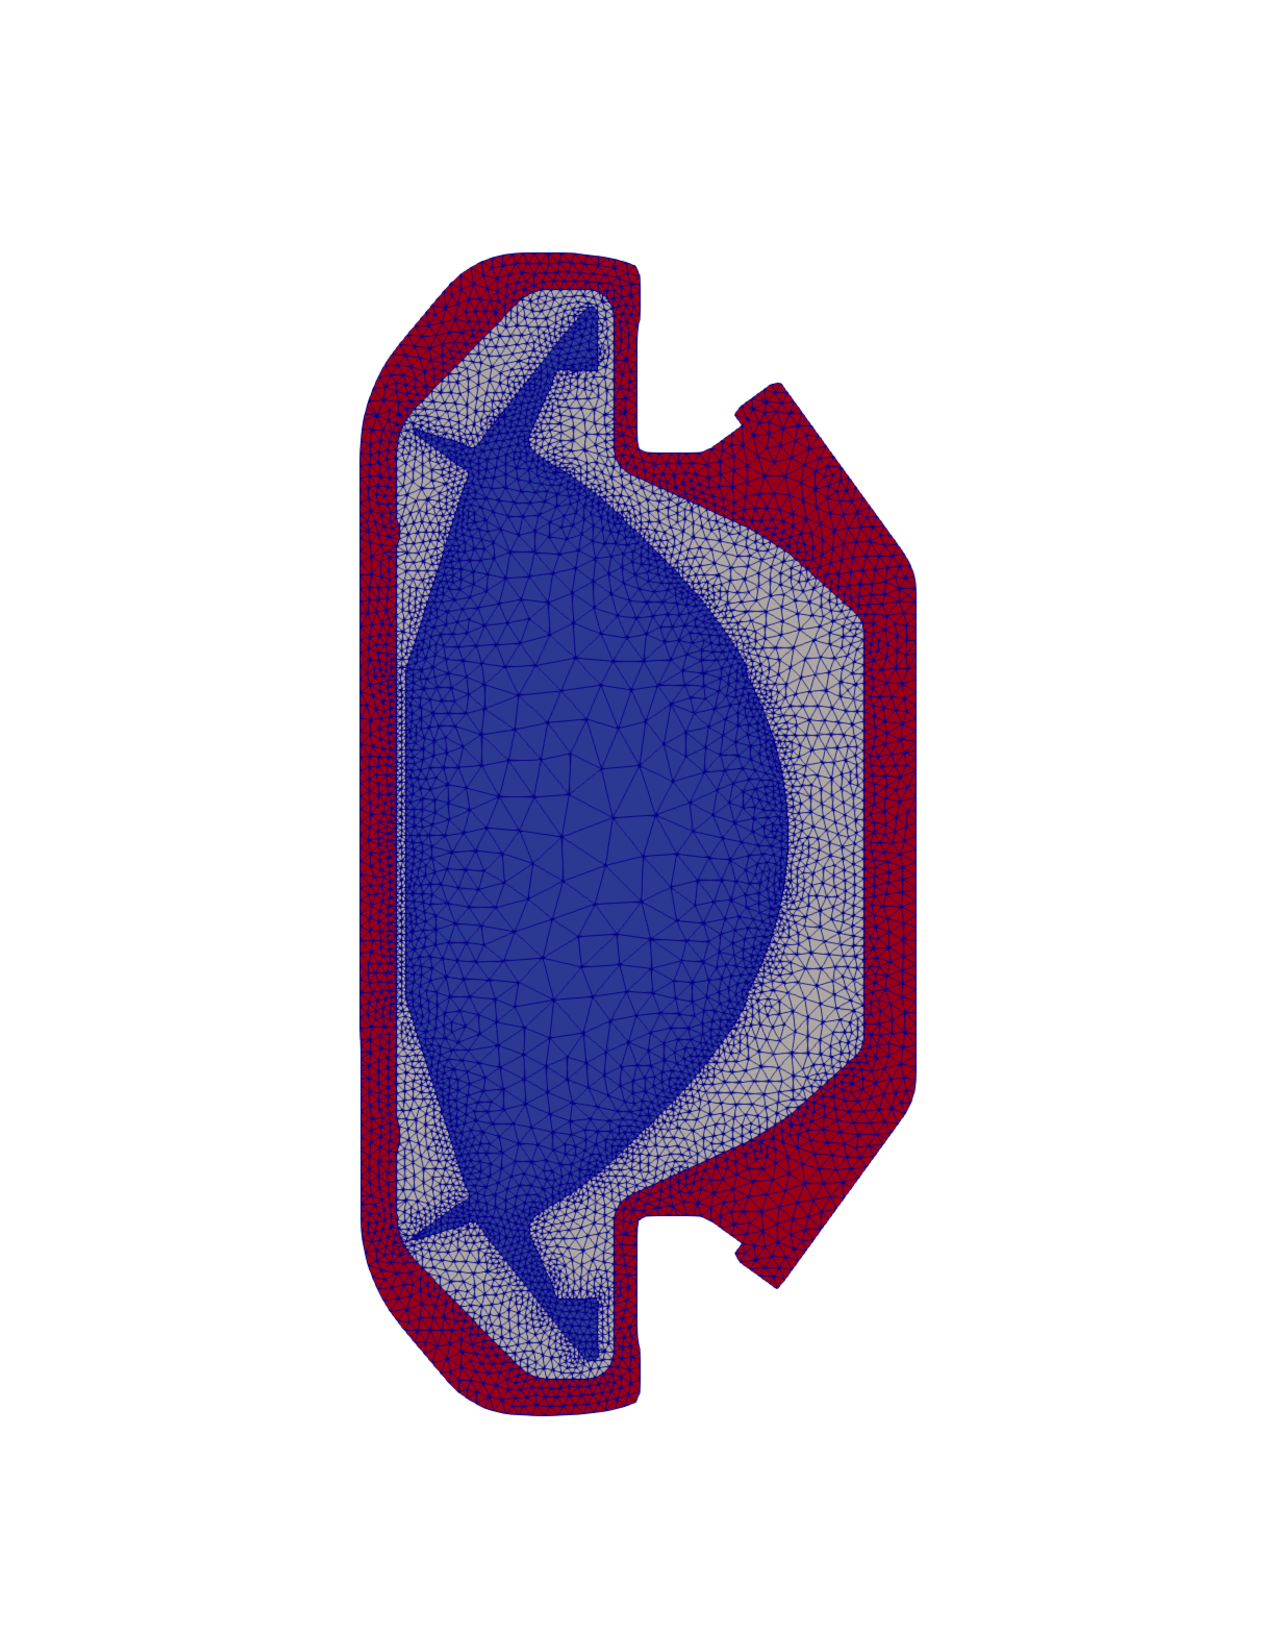
\includegraphics[width=3in]{./figures/meshgen-input3-novacuum.pdf}
\caption[Mesh with three boundary files and no vacuum wall]
{Mesh with three boundary files and no vacuum wall}
\label{fig:input3-novacuum}
\end{figure}

\begin{verbatim}
numBdry 3
bdryFile loop1.dat
bdryFile loop2.dat
bdryFile loop3.dat
numRgn 3
rgnBdry  1 1
rgnBdry  2 1 2
rgnBdry  2 2 3
outFile input3
meshSize 0.1 0.05 0.5
meshGradationRate 0.3
\end{verbatim}

The figure~\ref{fig:input3-novacuum} presents the mesh generated by the input file above.

\begin{figure}
\centering
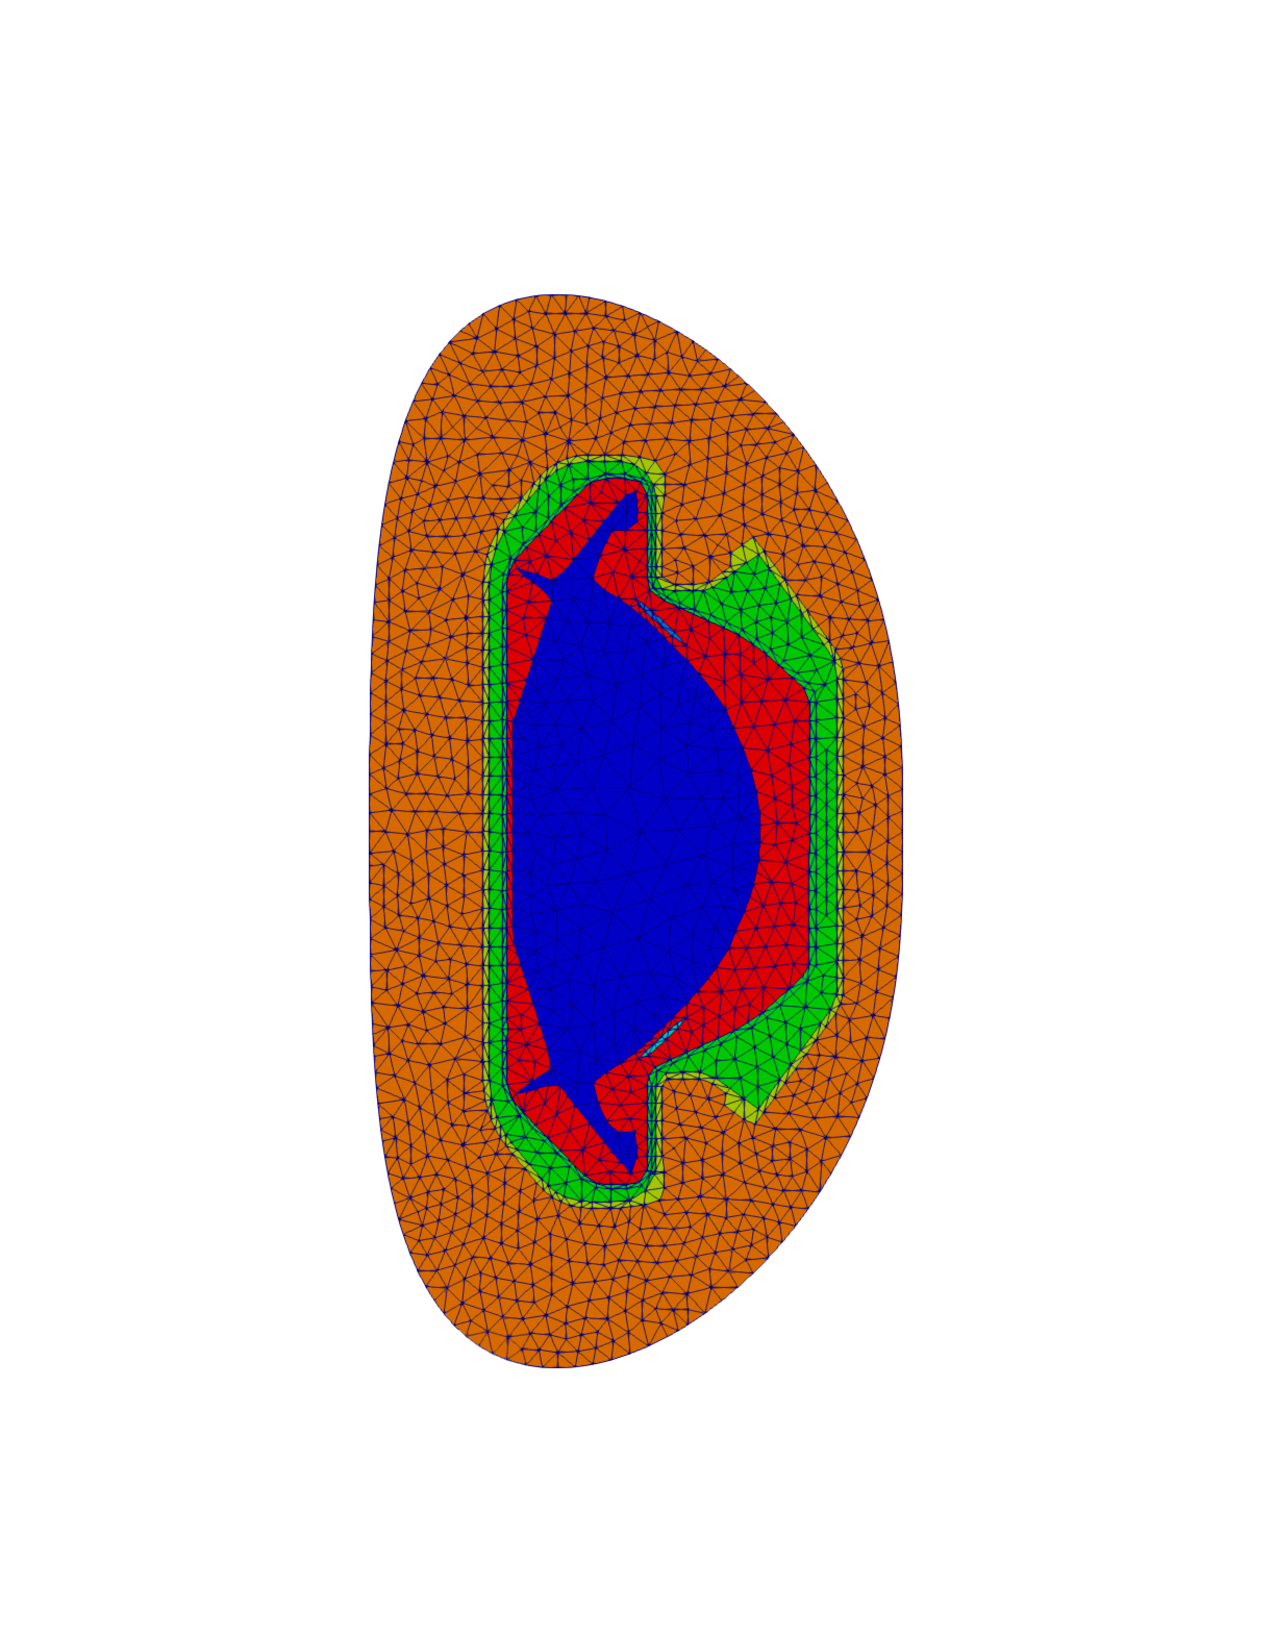
\includegraphics[width=3in]{./figures/meshgen-input7.pdf}
\caption[Mesh with seven boundary files and parameterized vacuum wall]
{Mesh with seven boundary files and parameterized vacuum wall}
\label{fig:input7-vacuum}
\end{figure}

\begin{verbatim}
numBdry 7
bdryFile loop1.dat
bdryFile loop2.dat
bdryFile loop3.dat
bdryFile loop4.dat
bdryFile loop5.dat
bdryFile loop6.dat
bdryFile loop7.dat
! if useVacuum=0, set numRgn to 7 and comment out [rgnBdry 4 1 2 3 4]
numRgn 8	
rgnBdry  1 1
rgnBdry  1 2
rgnBdry  1 3
rgnBdry  2 4 5
rgnBdry  2 5 6
rgnBdry  2 6 7
rgnBdry  2 7 8
rgnBdry  4 1 2 3 4
outFile input7
useVacuum 1
useVacuumParams 1
vacuumParams 1.8 1.5 0.4 0.0 2.5
numVacuumPts 20
! set meshSize for each region (default 0.05)
! e.g. for 3 region model, set three doubles for plasma, resistive, vacuum
meshSize 0.02 0.005 0.005 0.01 0.2 0.1 0.2 0.2 
\end{verbatim}

The figure~\ref{fig:input7-vacuum} presents the mesh generated by the input file above.


%%%%%%%%%%%%%%%%%%%%%%%%%%%%%%%%%%%%%%%%%
\subsubsection{polar\_meshgen}
%%%%%%%%%%%%%%%%%%%%%%%%%%%%%%%%%%%%%%%%%
\texttt{polar\_meshgen} requires an ascii file of arbitrary name that contains input parameters as the following:
\begin{itemize}
\item inFile: input file name containing equilibrium generation by jsolver
\item outFile: output file name to save model and mesh
\item meshSize: relative mesh size for each region (default 0.05)
\item reorder: if 1, reorder PUMI mesh based on adjacency (default: 0) and generate vtk folders for mesh visualization. The mesh before and after reodering is saved in \texttt{original-mesh.vtk} and \texttt{reordered-mesh.vtk}, respectively. Note that the element order of Simmetrix mesh is not affected.
\end{itemize}

The following presents an example input file ``\texttt{polar\_input}''.
\begin{verbatim}
inFile POLAR
outFile polar
meshSize 0.04
\end{verbatim}

To run \texttt{polar\_meshgen}, place \texttt{polar\_input} and \texttt{POLAR} in your work folder and do ``\texttt{polar\_meshgen polar\_input}''. The program will read \texttt{POLAR} and generate various model and mesh files starting with ``polar''. For instance, \texttt{polar-2K0.smb, pol-2K.sms, pol-2K.vtk, polar.dmg, polar.smd, polar.txt}. If the resulting mesh is too fine, increase the value of \texttt{meshSize}. If the resulting mesh is too coarse, decrease the value of \texttt{meshSize}. If \texttt{meshSize} is not specified in the input file, the default value is 0.05.   


%%%%%%%%%%%%%%%%%%%%%%%%%%%%%%%%%%%%%%%%%
\subsubsection{Example: Type 0 (parameterized vacuum)}
%%%%%%%%%%%%%%%%%%%%%%%%%%%%%%%%%%%%%%%%%

See the example input file \texttt{"analytic-input"}.


%%%%%%%%%%%%%%%%%%%%%%%%%%%%%%%%%%%%%%%%%
\subsubsection{Example: Type 1 (piece-wise linear vacuum)}
%%%%%%%%%%%%%%%%%%%%%%%%%%%%%%%%%%%%%%%%%

%%%%%%%%%%%%%%%%%%%%%%%%%%%%%%%%%%%%%%%%%
\subsubsection{Example: Type 2 (piece-wise polynomial vacuum)} 
%%%%%%%%%%%%%%%%%%%%%%%%%%%%%%%%%%%%%%%%%

See the example input file \texttt{"poly-input"}.

%%%%%%%%%%%%%%%%%%%%%%%%%%%%%%%%%%%%%%%%%
\subsubsection{Example: Type 3 (three-regions with inner wall points)}
%%%%%%%%%%%%%%%%%%%%%%%%%%%%%%%%%%%%%%%%%
See the example input file \texttt{"circle-input"}.

%%%%%%%%%%%%%%%%%%%%%%%%%%%%%%%%%%%%%%%%%
\subsubsection{Example: Type 4: (three-regions with inner $\&$ outer wall points)}
%%%%%%%%%%%%%%%%%%%%%%%%%%%%%%%%%%%%%%%%%
See the example input file \texttt{"bdry-input"}.

%%%%%%%%%%%%%%%%%%%%%%%%%%%%%%%%%%%%%%%%%
\subsubsection{Example: Multiple-regions with inner $\&$ outer wall points}
%%%%%%%%%%%%%%%%%%%%%%%%%%%%%%%%%%%%%%%%%
See the example input file \texttt{"multi-input"}.

%%%%%%%%%%%%%%%%%%%%%%%%%%%%%%%%%%%%%%%%%
\subsubsection{Example: Equilibrium}
%%%%%%%%%%%%%%%%%%%%%%%%%%%%%%%%%%%%%%%%%

The program \texttt{read\_jsolver} generates equilibrium and stores in the file \texttt{POLAR}. Given the input file \texttt{POLAR}, \texttt{m3dc1\_meshgen} generates the following files:
\begin{itemize}
\item	model.dmg: PUMI-readable model file
\item	model.txt: M3DC1-readable model file
\item	mesh0.smb: PUMI/M3DC1-readable mesh file
\item	mesh.vtk: Paraview data files
\item	norm\_curv: ascii file containing nodes' normal/curvature information
\end{itemize} 

%%%%%%%%%%%%%%%%%%%%%%%%%%%%%%%%%%%%%%%%%
\subsection{Mesh Control with SimModeler}
SimModeler is a graphical user interface to the Simmetrix geometry and mesh generation software. In cases where the currently available capabilities of m3dc1\_meshgen do not provide a satisfactory mesh, SimModeler can be used to apply alternative mesh control information to the Tokamak cross section geometry to generate different meshes. The information below indicates the application of a subset of the mesh controls that can be applied. For additional information of the full range of SimModeler mesh control options see: ********** FILL IN POINTER TO SIMMETRIX DOCUMENTATION *****
\label{ch:simmodeler}
%%%%%%%%%%%%%%%%%%%%%%%%%%%%%%%%%%%%%%%%%
(Contributed by D. Pfefferle on 4/27/16) On PPPL Portal, load a module \texttt{simmodeler} and run it.
\begin{enumerate}
\item From the menu \texttt{"File$\rightarrow$Open Model"}, load a model file (\texttt{.smd}) generated by \texttt{m3dc1\_meshgen}
\item In the upper panel, in the views section, click on \texttt{Front} to view the model, then go to \texttt{Meshing} tab
\item Select outer region, click \texttt{+} in \texttt{Mesh Attributes} and select \texttt{Mesh Size$\rightarrow$relative}. 
Enter a value (typically 0.1)
\item Select wall region, click \texttt{+} in \texttt{Mesh Attributes} and select \texttt{Mesh Size$\rightarrow$relative}. 
Enter a value (typically 0.02)
\item Select inner region, click \texttt{+} in \texttt{Mesh Attributes} and select \texttt{Mesh Size$\rightarrow$relative}. 
Enter a value (typically 0.04). Here, one can already generate the mesh by clicking on \texttt{Generate Mesh} and verify if the mesh sizes are suitable 
\item 	Select both inner and wall regions (holding shift key), click \texttt{+} in \texttt{Mesh Attributes} and select \texttt{Mesh Size$\rightarrow$relative}. Enter a function, e.g. \texttt{0.01$\times$abs(\$y+1.5)\^{}2+0.004} to specify an anisotropic mesh density on top of previous settings
\\ There are many available parameters for fine-tuning the mesh density.  For example, \texttt{Mesh Curvature Refinement} with parameter packs more elements near the edges of the resistive wall. 
\item \texttt{Generate Mesh} and \texttt{Show Mesh} to view result in new windows
\item If the result is satisfactory, from the menu \texttt{File$\rightarrow$Save Mesh}, give it a meaningful name with the extension \texttt{.sms}. The original model file \texttt{.smd} has been automatically saved by the program with your mesh modifications.
\item Close \texttt{simmodeler} then it will release a license. Until you quit Simmodeler, no one cannot run neither \texttt{m3dc1\_meshgen} nor \texttt{simmodeler}.
\item Copy the \texttt{.txt, .smd} and \texttt{.sms} files to the simulation directory and run the following splitting routine to obtain PUMI-readable \texttt{.smb} mesh files.
\newline\newline
\texttt{/p/tsc/C1/m3dc1-sunfire.r6-1.5/bin/part\_mesh.sh model\_file.smd mesh\_file.sms X}, 
where \texttt{X} is the number of parts you need in the \texttt{.smb} mesh.
\item Modify the \texttt{C1input} file accordingly
\newline\newline
\texttt{mesh\_filename = `part.smb'
\\
mesh\_model = `filename.txt'
}
\end{enumerate}

%%%%%%%%%%%%%%%%%%%%%%%%%%%%%%%%%%%%%%%%%
\subsection{Mesh Partitioning}
\label{ch:mesh-ptn}
%%%%%%%%%%%%%%%%%%%%%%%%%%%%%%%%%%%%%%%%%

\subsubsection{Splitting}

The program \texttt{split\_smb} increases the number of parts in a mesh from \texttt{P} to \texttt{N} (\texttt{P$<$N}). 
In each machine, the program \texttt{split\_smb} is availble in \texttt{\$SCOREC\_UTIL\_DIR} provided in \texttt{hostname.mk} file.

In order to split \texttt{P}-part mesh to \texttt{N} parts (\texttt{N$>$P}), run
\texttt{"mpirun -np N ./split\_smb input-mesh(.smb) output-mesh(.smb) X"}
\begin{itemize}
\item	the file extension of input-mesh should be .smb 
\item	the file extension of output-mesh should be .smb
\item	\texttt{N} is the number of parts in the output mesh
\item	For a \texttt{P}-part input mesh, \texttt{X} must be \texttt{N/P}
\item	For both input and output mesh, do not specify a number before the file extension
\item	\texttt{split\_smb} will insert a number in the output mesh file. The number represents a global part ID.
\item	Make sure that the output mesh doesn't have any empty part. Otherwise, the program crashes with the following error message:
\newline
\texttt{APF warning: 1 empty parts}
\newline
\texttt{split\_smb: \ldots/mds/mds.c:614: check\_ent: Assertion `e $>$= 0' failed}
\end{itemize}

Examples on portal:
\begin{enumerate}
\item To split a serial (1-part) mesh to 6 parts, run\\
 \texttt{"mpirun -np 6 ./split\_smb struct-curveDomain.smb part.smb 6"}
\begin{itemize}
\item	Input mesh: struct-curveDomain0.smb 
\item	Output mesh: part0.smb, part1.smb, part2.smb, part3.smb, part4.smb, part5.smb
\end{itemize}

\item To split a 2-part mesh to 6 parts, run
 \texttt{"mpirun -np 6 ./split\_smb  struct-curveDomain.smb part.smb 3"}
\begin{itemize}
\item	Input mesh: struct-curveDomain0.smb, struct-curveDomain1.smb
\item	Output mesh: part0.smb, part1.smb, part2.smb, part3.smb, part4.smb, part5.smb
\end{itemize}
\end{enumerate}

See \texttt{readme.split\_smb} for detailed instructions and trouble shooting tips.

%%%%%%%%%%%%%%%%%%%%%%%%%%%%%%%%%%%%%%%%%
\subsubsection{Mesh Merging}
\label{ch:mesh-mg}
%%%%%%%%%%%%%%%%%%%%%%%%%%%%%%%%%%%%%%%%%

The program \texttt{collapse} decreases the number of parts in a mesh from \texttt{N} to \texttt{P} (\texttt{P$<$N}). 
In each machine, the program \texttt{collapse} is availble in \texttt{\$SCOREC\_UTIL\_DIR} provided in \texttt{hostname.mk} file.

In order to merge \texttt{N}-part .smb mesh to \texttt{P} parts (\texttt{P$>$0}), run
\texttt{"mpirun -np N ./collapse input-mesh(.smb) output-mesh(.smb) X"}
\begin{itemize}
\item	the file extension of input-mesh should be .smb 
\item	the file extension of output-mesh should be .smb
\item	\texttt{N} is the number of parts in the input mesh
\item	For a \texttt{P}-part output mesh, \texttt{X} must be \texttt{N/P}
\item	For both input and output mesh, do not specify a number before the file extension
\item	\texttt{collapse} will insert a number in the output mesh file. The number represents a global part ID.
\end{itemize}

Example on portal:
\newline
In order to merge 4-part mesh into a serial (1-part) mesh, run
\texttt{"mpirun -np 4 ./collapse part.smb serial.smb 4"}
\begin{itemize}
\item	Input mesh: part0.smb, part1.smb, part2.smb, part3.smb
\item	Output mesh: serial0.smb
\end{itemize}

See \texttt{readme.collapse} for detailed instructions and trouble shooting tips.
